% !Mode:: "TeX:UTF-8"

\section{狭义相对论: 物理规律以闵氏几何为时空背景}

\subsection{间隔不变及其导致的时空特征, 狭义相对性原理}

\subsubsection{光速/间隔不变, 间隔/时空的划分, 因果律}

实验发现, 在任何惯性系中, 光速不仅是一切物体发生运动--亦即一切联系讯号--所可能具有的最大速度, 而且是不变的. 于是, 对两个用光速联系着的事件, 可知它们之间的如下量
\begin{align}
ds^2:=c^2dt^2-d\bm{r}^2
\end{align}
在任何惯性系中都是为零的, 从而是相等的. 而若两个事件是用低于或高于光联系着的, 它们间的此量便不再为零; 但由等价性不难看出, 在不同惯性系中看来, 它们仍是相等的. 我们将上述量命名为两个事件间的间隔. 若再命
\begin{gather}
x^\mu:=(x^0,x^i)=(x^0,x^1,x^2,x^3)=(ct,x,y,z)=(ct,\bm{r}),\\
x_\mu:=(x^0,x_i)=(x_0,x_1,x_2,x_3)=(ct,-x,-y,-z)=(ct,-\bm{r}),
\end{gather}
则可将间隔表为
\begin{gather}
ds^2=dx_\mu dx^\mu=g_{\mu\nu}dx^\mu dx^\nu;
\end{gather}
其中
\begin{align}
g^{\mu\nu}=g_{\mu\nu}=\left[\begin{array}{cccc}1&0&0&0\\0&-1&0&0\\0&0&-1&0\\0&0&0&-1\end{array}\right]:=\rm{diag}(+,-,-,-)
\end{align}
称为度规. 由度规的出现可以看出, 狭义相对论事实上是关于物理规律的时空背景的几何理论--广义相对论亦是如此. 本度规所描述的时空/几何, 称为闵氏时空/几何; 由此度规所描述的时空, 我们称为平直时空. 事实上, 给定了度规, 就完全确定了某时空的基本性质. 以后我们将具体展现.


间隔不变性刻画了时空的一种绝对划分: 对某一个事件--我们假设它在原点处, --当另外事件与之分别是用大于/等于/小于光速的速度值联系着的时候, 那么在任何参照系下它们都是用大于/等于/小于光速的速度值联系着的. 我们把这三种间隔, 分别称为类空的, 类光的以及类时的. 即对任意惯性系变换, 某种间隔内事件只在本间隔内变换, 而不会外出.


稍后不难确证, 对于有着非类空间隔的两件事, 对不同的参照系, 它们的先后次序~(即间隔的时间分量) 仍是不变的; 而有着类空间隔的两件事, 如同时发生的两件事, 它们的先后将随参照系的不同而不同. 这意味着, 非类空间隔的两件事可以建立因果联系, 类空间隔的两件事不可能建立因果关系. 这称为狭义相对论所界定的微观世界的因果律.
\begin{figure}[!h]
\begin{center}
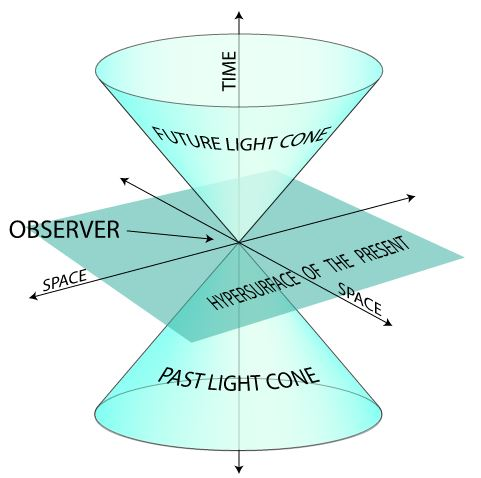
\includegraphics[width=4.2 cm]{pic/space.jpg}
\caption{间隔/时空区域的划分.}
\label{space}
\end{center}
\end{figure}


\subsubsection{惯性变换/洛伦兹~boost}

设坐标系~$\Sigma'$ 与~$\Sigma$ 的三轴分别平行, 前者沿后者~$x$ 轴的负方向以速度~$v$ 运动; 那么, 由光速不变性或由其进一步导致的间隔不变性, 一个事件, 若在~$\Sigma$ 系看来坐标是~$x^\mu=(ct, x, y, z)$, 则在~$\Sigma'$ 系看来其坐标就是
%\begin{equation}
%\left\{
%\begin{array}{l}
%ct'=\frac{ct+\frac{v}{c}x}{\sqrt{1-\frac{v^2}{c^2}}},\\
%x'=\frac{vt+x}{\sqrt{1-\frac{v^2}{c^2}}},\\
%y'=y,\\
%z'=z;
%\end{array}
%\right.
%\end{equation}
\begin{equation}
\left\{
\begin{aligned}
ct'&=\frac{ct+\frac{v}{c}x}{\sqrt{1-\frac{v^2}{c^2}}},\\
x'&=\frac{vt+x}{\sqrt{1-\frac{v^2}{c^2}}},\\
y'&=y,\\
z'&=z;
\end{aligned}
\right.
\end{equation}
上述变换即同一事件在不同惯性系中的变换式, 亦称为洛伦兹变换在~$x$ 方向上的~boost. 我们还可将上述变换用矩阵形式表为
\begin{align}
\left[
\begin{array}{l}
ct'\\x'\\y'\\z'
\end{array}
\right]=
\left[
\begin{array}{cccc}
\gamma&\beta\gamma&0&0\\
\beta\gamma&\gamma&0&0\\
0&0&1&0\\
0&0&0&1
\end{array}
\right]
\left[
\begin{array}{l}
ct\\x\\y\\z
\end{array}
\right];
\end{align}
其中已命
\begin{align}
\gamma=\frac{1}{\sqrt{1-\frac{v^2}{c^2}}},~\beta=\frac{v}{c}.
\end{align}
显然, 有~$\gamma^2-(\beta\gamma)^2=1$.



最后, 我们不难写出洛伦兹惯性变换的矢量表达式:
\begin{gather}
t'=\gamma\left(t+\frac{\bm{r}\cdot\bm{v}}{c^2}\right),\\
\bm{r}'=\bm{r}+(\gamma-1)r_v\bm{v}^0+\gamma t\bm{v}.
\end{gather}

\subsubsection{四维量的协变性与三维量的相对性: 间隔膨胀, 长度收缩, 同时相对}


由洛伦兹变换可见, 某事件的时间间隔, 或某物体的长度/体积, 若在固定于它身上的坐标系--取为~$\Sigma'$--看来是~$\Delta\tau,~l_0$ 或~$V_0$, 称为固有时, 固有长度等, 则在~$\Sigma$ 看来就是
\begin{gather}
\Delta t=\gamma_0\Delta\tau,~l=l_0/\gamma_0,~dV=dV_0/\gamma_0.
\end{gather}
显然, 因为时间, 长度与体积等并不是四维量, 而只是作为四维标量的间隔~$ds^2$ 的一部分, 所以在不同参考系下它们的值将发生变化, 自然是不奇怪的. 事实上, 包括我们稍后要讲到的电磁学, 它们的相对论效应, 就出在我们对作为四维协变量的分量化观察之中.

%上述, 是考察在动系看来, 物体本身为系, 这样子的变化的; 当然, 也可以考察一个长度, 时间, 或体积, 任意两个动系间看起来它们的变化情况, 但, 这意义不大.


%在我中静止的物体, 我看, 与动者看, 我是大的, 动者看是小的.

\subsubsection{狭义相对性原理: 物理规律四维协变}

我们相信, 一切惯性系都应是等价在, 物理规律在何任惯性系中都应被表为相同的形式. 具体操作上讲, 这要求物理规律方程中的出现的每个物理量, 都应是洛伦兹协变量. 这, 称为狭义相对性原理. 它与光速不变事实一起, 就可揭示出关于我们这个世界的很多以前不为人知的事实. 而当然, 此理论的正确性, 也由这些事实的被发现得以确证.


\subsection{力学的洛伦兹协变性; 新发现: 能动关系与质能等价}

力学的以伽利略变换作为时空背景的牛顿表述, 显然不具有洛伦兹不变性. 那么首先, 我们来构造洛伦兹协变的力学规律. 我们定义四维速度:
\begin{align}
u^\mu:=\frac{dx^\mu}{d\tau}=\gamma_0\frac{dx^\mu}{dt}=\gamma_0(c,\bm{u}).
\end{align}
下面我们证明, 此量的确是一个协变的洛伦兹矢量. 我们知道, 对任意空度规空间, 与其中坐标有着相同变换关系的量, 称为矢量. 于是证明~$u^\mu=\gamma_0(c,\bm{u})$ 为洛伦兹矢量, 等价于证明~$c\gamma'_0=\gamma(c\gamma_0+\beta u_x\gamma_0)$ 或~$u'_x\gamma'_0=\gamma(\beta c\gamma_0+u_x\gamma_0)$. 注意其中我们已取~$u^1=\gamma_0 u_x$. 由前述洛伦兹~boost 我们可以直接推得三维速度矢量的变换式为\footnote{由此亦可得出~$\gamma=\gamma_0\gamma'_0(1-\beta_0\beta'_0)$.}
\begin{align}
u'_x=\frac{u_x+v}{1+\frac{u_x v}{c^2}};
\end{align}
而可以发现, 此式与前述待证明的两式是互致的. 于是~$u^\mu$ 是洛伦兹矢量得证. 另外, 两个洛伦兹矢量得到一个洛伦兹标量; 如果四维速度矢量作如上定义的话, 这就是~$\gamma_0^2c^2-\gamma_0^2u^2=c^2$; 而此式的确是成立的. 于是再一次辅证了~$u^\mu$  的洛伦兹矢量性.\footnote{本段分析亦表明, 不像~$(x,y,z)$ 仍是四维协变坐标的三维分量, $\gamma_0 u_x,~\gamma_0 p_x$ 才是四维速度/四维动量的三维分量. 这也就意味着, 我们对牛顿理论中的速度与动量的定义作了改造.%: 在低速三维情况时, 不像坐标仍可精确表为~$(x,y,z)$, 速度与动量等表述为~$\gamma_0 u_x$ 或~$\gamma_0 p_x$ 才是精确的; 只在速度或动量为零, 即物体静止时, 才有~$\gamma_0 p_x=p_x$ 回到牛顿理论中的定义.
}


有了以上之铺垫, 洛伦兹协变的动量四维矢量就可定义为
\begin{align}
p^\mu:=m_0u^\mu=(\gamma_0 m_0c,\gamma_0 m_0\bm{u})=(\frac{\gamma_0 m_0c^2}{c},\bm{p})=(\frac{E}{c},\bm{p})
\end{align}
(由此可看出~$Et-\bm{p}\cdot\bm{r}=p^\mu x_\mu$ 是四维标量); 上式中取~$E=\gamma_0 m_0c^2$ 的原因, 是作泰勒展开可以发现~$\gamma_0 m_0c^2=m_0c^2+\frac{1}{2}m_0v^2+\cdots$. 于是我们发现, 当物体静止时, 仍有~$E_0=m_0c^2$ 的能量, 这称为质能等价; 而~$\frac{E^2}{c^2}-\bm{p}^2=m_0^2c^2$, 即
\begin{align}
E^2=\bm{p}^2c^2+m_0^2c^4,
\end{align}
称为能动关系. 刚才已经知道, 矢量与坐标有着相同变换关系. 所以, 例如对于动量, 假设两系沿~$i$ 轴运动, 我们就有~(已采用自然单位):
\begin{gather}\label{titi}
E'=\gamma(E+\beta p^i),~p'^i=\gamma(\beta E+p^i).
\end{gather}
不难上述第一式, 作为早先发现的~$E=\gamma_0E_0$~或~$E'=\gamma'_0E_0$ 的更一般的推广, 的确是可以给出后二者及其关系的: $\gamma'_0E_0=\gamma(\gamma_0E_0+\beta E_0u_x\gamma_0)\rightarrow\gamma'_0=\gamma(\gamma_0+\beta u_x\gamma_0)$.

最后, 我们把牛顿力学改造洛伦兹协变的版本. 首先我们定义~$F^\mu:=\frac{dp^\mu}{d\tau}$. 考察此四维力的空间分量, 得出~$\bm{F}=\frac{d\bm{p}}{d\tau}$; 其中三维动量的定义与前文是一致的, 即~$\bm{p}=\gamma_0m_0\bm{u}$; 相似地, 四维力的三维空间分量, 相比较牛顿理论中的, 亦是被作了改造的. 考察四维力的零分量, 得出~$F^0=\frac{dp^0}{d\tau}=\frac{1}{c}\frac{dE}{d\tau}=\frac{1}{c}\frac{c^2\bm{p}}{E}\cdot\frac{d\bm{p}}{d\tau}=\frac{\bm{u}\cdot\bm{F}}{c}$; 注意其中~$c^2\bm{p}=E\bm{u}$. 于是最终我们获得~$F^\mu=(\frac{\bm{F}\cdot\bm{u}}{c},\bm{F})$.






\subsection{电磁学的相对论效应, 电动力学的洛伦协协变性}
\subsubsection{光的多普勒效应与光行差的严格公式}
经典的波与动运物体, 就可能出现多普勒效应与~``行差'' 现象; 但光的多普勒效应与光行差现象, 只有使用狭义相对论, 才能给出严格结果. 这些效应, 当然出在我们对四维波矢的分量化观察之中. 下面我们具体考察之.

首先, 不难明确, 相位因子~$\omega t-\bm{k}\cdot\bm{r}$ 应该是洛伦兹标量. 如此, 如下构造四维波矢就是合适的~$k^\mu=(\frac{\omega}{c},\bm{k})$. 由此我们可以得出~$\ frac{\omega'}{c}=\gamma(\frac{\omega}{c}+\beta k_x),~k'_x=\gamma(\beta\frac{\omega}{c}+k_x)$; 若再设~$\bm{k}',~\bm{k}$ 与~$x$ 轴正方向的夹角分别为~$\theta',~\theta$, 即~$k_x=\frac{\omega}{c}\cos\theta,~k'_x=\frac{\omega}{c}\cos\theta'$-- 其中用到了~$\omega=kc$, 则前两式变成
\begin{gather}
\omega'=\omega\gamma\left(1+\frac{v}{c}\cos\theta\right),\tan\theta'=\frac{\sin\theta}{\gamma\left(\cos\theta+\frac{v}{c}\right)};
\end{gather}
此即相对应效应多普勒公式与光行差公式. 进一步地, 我们设光源静止于~$\Sigma'$ 系, $\omega'=\omega_0$ 即光源自己来看的辐射角频律, 于是
\begin{align}
\omega=\frac{\omega_0}{\gamma\left(1+\frac{v}{c}\cos\theta\right)}
\end{align}
即~$\Sigma$ 系中的观测者测出的角频; 其中~$\theta$ 即观测者看到的辐射方向与光源运动方向的夹角. 由此可以看出光的多普勒效应的经典公式的确作为上式的低速近似出现. 另外, 在垂直于光源运动方向的方向上, 相对论公式给出~$\omega=\omega_0\sqrt{1-\frac{v^2}{c^2}}$; 此效应称为横向多普勒效应. 作为比较, 此情况下多普勒效应经典公式仍给出~$\omega=\omega_0$, 即未能预言出应有的现象. 这进一步说明经典理论的不足以及相对论的正确性.










我们将看到, 不同于力学牛顿理论的需要被改造, 电磁学背后的动力学规律, 即电动力学, 或具体地说即麦克斯韦方程组, 是相对论协变的. 接下来我们重点研究之.

\subsubsection{麦克斯韦方程组的四维协变形式}
麦克斯韦方程组的三维矢量式为
\begin{gather}
\nabla\cdot\bm{E}=\frac{\rho}{\epsilon_0},\\
\nabla\times\bm{B}=\mu_0\bm{J}+\mu_0\epsilon_0\frac{\partial\bm{E}}{\partial t},\\
\nabla\cdot\bm{B}=0,\\
\nabla\times\bm{E}=-\frac{\partial\bm{B}}{\partial t};
\end{gather}
其中~$c=\frac{1}{\sqrt{\mu_0\epsilon_0}}$, 是光速. 我们可以引入矢势与标势, 有
\begin{gather}
\bm{B}=\nabla\times\bm{A},~\bm{E}=-\nabla\varphi-\frac{\partial\bm{A}}{\partial t}.
\end{gather}
下面我们要找出麦克斯韦方程组的四维形式. 为此, 将以上两式用分量形式写出, 即~$B^i=\partial_jA^k-\partial_kA^j,~E^i=-\partial_icA^0-c\partial_0A^i$; 其中构造了~$A^\mu=(\frac{\varphi}{c},\bm{A})$, 以及~$\partial_\mu:=\frac{\partial}{\partial x^\mu}=(\partial_0,\partial_i)=(\frac{\partial}{\partial t},\nabla)$. 进一步变形及命令, 可得:
\begin{align}
-B^i&=\partial^jA^k-\partial^kA^j:= F^{jk},\\
-\frac{E^i}{c}&=\partial^0A^i-\partial^iA^0:= F^{0i};
\end{align}
此即意味着场强与势的关系可合写为并列出分量值为:
\begin{align}
F^{\mu\nu}=\partial^\mu A^\nu-\partial^\nu A^\mu=
\left[
\begin{array}{cccc}
0&-E_x/c&-E_y/c&-E_z/c\\
E_x/c&0&-B_z&B_y\\
E_y/c&B_z&0&-B_x\\
E_z/c&-B_y&B_x&0
\end{array}
\right].
\end{align}
其中~$F^{\mu\nu}$ 即由~$\bm{E}$ 与~$\bm{B}$ 构成的电磁场张量. 显然, 上述逆变形式的电磁场张量是反对称的. 我们还可写出电磁场张量的其它形式, 如混合张量
\begin{align}
{F^\mu}_\nu=\partial^\mu A_\nu-\partial^\nu A_\mu=F^{\mu\alpha}g_{\alpha\nu}=
\left[
\begin{array}{cccc}
0&E_x/c&E_y/c&E_z/c\\
E_x/c&0&B_z&-B_y\\
E_y/c&-B_z&0&B_x\\
E_z/c&B_y&-B_x&0
\end{array}
\right].
\end{align}
相应地, 我们可将麦克斯韦方程组分别表为
\begin{gather}
\partial_xF^{x0}+\partial_yF^{y0}+\partial_zF^{z0}=\partial_iF^{i0}=\mu_0 J^0,\\
\partial_jF^{ji}+\partial_kF^{ki}+\partial_0F^{0i}=\partial_jF^{ji}+\partial_0F^{0i}=\mu_0J^i,\\
\partial_iF_{jk}+\partial_jF_{ki}+\partial_kF_{ij}=0,\\
\partial_jF^{k0}+\partial_kF^{0j}-\partial_0F^{jk}=0;
\end{gather}
其中作了构造\footnote{同时~$J^\mu=\rho_0 u^\mu=\rho_0\gamma_0(c,\bm{u})$, 对比知~$\rho=\rho_0\gamma_0$; 这恰好补偿了体积的变化~$dV=dV_0/\gamma_0$, 使总电荷~$Q=\int dV\rho$ 保持为洛伦兹标量. 另外, 可见电荷守恒定律~$\frac{\partial\rho}{\partial t}+\nabla\cdot\bm{J}=\partial_\mu J^\mu=0$ 是洛伦兹不变的.}~$J^\mu=(c\rho,\bm{J})$. 上述方程前两式与后两式可进一步分别合写为
\begin{gather}
\partial_\mu F^{\mu\nu}=\mu_0J^\nu,\\
\partial_\mu F_{\nu\rho}+\partial_\nu F_{\rho\mu}+\partial_\rho F_{\mu\nu}=0;
\end{gather}
此即麦克斯韦方程组的四维协变形式. 由此我们知晓, 电磁学规律天生就是四维协变的.% 另外, 能导出电磁场的拉氏密度是~$\mathcal{L}=\frac{1}{4}F_{\mu\nu}F^{\mu\nu}$.
另外还可读出, 麦氏方程前两式是独立的, 而后两式, 作为~Bianchi 恒等式, 是~$F^{\mu\nu}$ 自然的拓扑性质.

我们知道对任何一个二阶张量都有~$T_{\mu\nu}=\frac{1}{2}(T_{\mu\nu}+T_{\mu\nu})+\frac{1}{2}(T_{\mu\nu}-T_{\mu\nu})\equiv T_{(\mu\nu)}+T_{[\mu\nu]}$, 即任一二阶张量都可由一个对称张量与一个反对称张量构成; 如对电磁场张量我们有~$F_{[\mu\nu]}=F_{\mu\nu}$. 如果我们如下定义一个三阶张量的全反对称张量: $T_{[\rho\mu\nu]}=\frac{1}{6}(T_{\rho\mu\nu}+T_{\mu\nu\rho}+T_{\nu\rho\mu}-T_{\rho\nu\mu}-T_{\nu\mu\rho}-T_{\mu\rho\nu})$, 则可知
\begin{gather}
\partial_{[\rho}F_{\mu\nu]}=\frac{1}{3}(\partial_\mu F_{\nu\rho}+\partial_\nu F_{\rho\mu}+\partial_\rho F_{\mu\nu})=0;
\end{gather}
上式可为麦克斯韦方程第二式的另一写法.

\subsubsection{势的规范冗余, 达朗贝尔方程的四维协变式}

容易推导出电磁势满足
\begin{gather}
\nabla^2\bm{A}-\frac{1}{c^2}\frac{\partial^2\bm{A}}{\partial t^2}-\nabla\left(\nabla\cdot\bm{A}+\frac{1}{c^2}\frac{\partial\varphi}{\partial t}\right)=-\mu_0\bm{J},\\
\nabla^2\varphi+\frac{\partial}{\partial t}\nabla\cdot\bm{A}=-\frac{\rho}{\epsilon_0}
\end{gather}
称为达朗贝尔方程. 由前述势与场强的关系表达式可以看出, 场强在以下两式进行协同变换--称为规范变换--时保持不变:
\begin{gather}
\bm{A}\rightarrow\bm{A}'=\bm{A}+\nabla\gamma,~\varphi\rightarrow\varphi'=\varphi-\frac{\partial\gamma}{\partial t};
\end{gather}
用四维语言叙述上两式合成~$A^\mu\rightarrow A'^\mu=A^\mu-\partial^\mu\gamma$. 也就是说, $(\frac{\varphi}{c},\bm{A})$ 与~$(\frac{\varphi'}{c},\bm{A}')$ 描述的是同一个物理实体. 势的这种规范冗余, 意味着我们可以给它加上条件, 称为规范条件. 常见的有库仑规范~$\nabla\cdot\bm{A}=0$, 与洛伦茨规范~$\nabla\cdot\bm{A}+\frac{1}{c^2}\frac{\partial\varphi}{\partial t}=\partial_\mu A^\mu=0$. 显然洛伦茨规范条件是协变的; 其下势方程化为
\begin{gather}
\nabla^2\bm{A}-\frac{1}{c^2}\frac{\partial^2\bm{A}}{\partial t^2}=-\mu_0\bm{J},~\nabla^2\varphi-\frac{1}{c^2}\frac{\partial^2\varphi}{\partial t^2}=-\frac{\rho}{\epsilon_0};
\end{gather}
上两式可合写为~$\partial^2 A^\mu=-\mu_0 J^\mu$, 显然亦是协变的.

当采取库仑规范时, 有~$\nabla^2\varphi=-\frac{\rho}{\epsilon_0}$. 对于自由场, 就得到~$\varphi=0$. 此式连同库仑规范条件, 称为辐射规范. --有人亦将之称为库仑规范. 在辐射规范下, 势方程就变为~$\partial^2\bm{A}=0$.

辐射规范的两个条件, 将电磁场的自由度由~4 降到了~2; 具体地, 对于平面波, 本规范给出~$\bm{k}\cdot\bm{A}=0$; 也即电磁场只有两个横向分量是自由有的, 没有纵向分量. 这, 与我们熟知的事实是一致的. 但是, 当然, 此规范是不具有洛伦兹协变性的. 如上所见, 洛伦茨规范倒是洛伦兹协变的, 但却不能消除所有非物理自由度.




\subsubsection{麦克斯韦方程组用微分形式表达}

电磁势用微分形式写出就是~$A=A_\mu dx^\mu$, 是一个~1-形式; 于是可以看出, 由其得出的如下~2-形式:
\begin{align}
F=dA=\partial_{[\mu}A_{\nu]}dx^\mu\wedge dx^\nu=\frac{1}{2}(\partial_\mu A_\nu-\partial_\nu A_\mu)dx^\mu\wedge dx^\nu=\frac{1}{2}F_{\mu\nu}dx^\mu\wedge dx^\nu,
\end{align}
即电磁场强; $F_{\mu\nu}$ 即电磁场张量. 我们知道外微分算符~$d$ 总有~$d^2=0$, 此即给出麦克方程第二式~$\partial_{[\rho}F_{\mu\nu]}=0$. 具体地,
\begin{gather}
dF=d^2A=\frac{1}{2}\partial_{[\rho}F_{\mu\nu]}dx^\rho\wedge dx^\mu\wedge dx^\nu=0.
\end{gather}
利用~Hodge 星算符\footnote{
利用此算符的定义~$\star(dx^{i_1}\wedge\cdots\wedge dx^{i_p})=\frac{1}{q!}{\epsilon_{j_1\cdots j_q}}^{i_1\cdots i_p}dx^{j_1}\wedge\cdots\wedge dx^{j_q}$, 可求得
\begin{gather}
\star dt=dx^i\wedge dx^j\wedge dx^k,~\star dx^i=dt\wedge dx^j\wedge dx^k;\\
\star (dt\wedge dx^i)=-dx^j\wedge dx^k,~\star(dx^i\wedge dx^j)=dt\wedge dx^k.
\end{gather}
%\begin{gather}
%\star dt=dx\wedge dy\wedge dz,~\star dx=dt\wedge dy\wedge dz,~\star dy=dt\wedge dz\wedge dx,~\star dz=dt\wedge dx\wedge dy;\\
%\star (dt\wedge dx)=-dy\wedge dz,~\star(dt\wedge dy)=-dz\wedge dx,~\star(dt\wedge dz)=-dx\wedge dy,\\
%\star(dx\wedge dy)=dt\wedge dz,~\star(dz\wedge dx)=dt\wedge dy,~\star(dy\wedge dz)=dt\wedge dx.
%\end{gather}
}~$\star$, 可求出
\begin{align}
d\star F=&d\star\left(\frac{1}{2}F_{\mu\nu}dx^\mu\wedge dx^\nu\right)\nonumber\\
=&d\star\left(F_{0i}dx^0\wedge dx^i+\frac{1}{2}F_{ij}dx^i\wedge dx^j\right)\nonumber\\% 这是总项
=&d\left(F_{i0}dx^j\wedge dx^k+F_{ij}dx^0\wedge dx^k\right)\nonumber\\%这里变成了单项, 需要循环相加
=&\partial_iF_{i0}dx^i\wedge dx^j\wedge dx^k+\partial_iF_{ij}dx^i\wedge dx^0\wedge dx^k\nonumber\\
=&-\mu_0\star J_0dx^0+\mu_0\star J_jdx^j\nonumber\\
=&-\mu_0\star J;
\end{align}
其中~$J=J_\mu dx^\mu$ 为一个~1-形式. 显然, 上述式子即麦氏方程前两式之合写.
%\begin{align}
%d\star F=&d\star\left(\frac{1}{2}F_{\mu\nu}dx^\mu dx^\nu\right)\\
%=&d\star(F_{01}dx^0\wedge dx+F_{02}dx^0\wedge dy+F_{03}dx^0\wedge dz\\
%&+F_{12}dx\wedge dy+F_{31}dz\wedge dx+F_{23}dy\wedge dz)\\
%=&d(-F_{01}dy\wedge dz-F_{02}dz\wedge dx-F_{03}dx\wedge dy\\
%&+F_{12}dt\wedge dz+F_{31}dt\wedge dy+F_{23}dt\wedge dx)\\
%=&-\mu_0\star J.
%\end{align}



\subsection{洛伦兹群表示论}%: 场的性质~(标量/矢量/旋量) 与粒子自旋的关系--Wigner 定理; 旋量, 狄拉克方程的严格导出, 物理规律的~$CPT$ 离散变换性质}

闵氏时空的对称群, 是洛伦兹/庞加莱群; 前者的几何性质由后者精确体现. 特别地, 对洛伦兹群表示理论的研究, 将使我们看到作为群的表示基的场函数的自旋的出现, 以及后者与场的性质的对应关系; 还可使我们发现旋量, 并严格推导出旋量满足的狄拉克方程. 我们还将仔细探讨物理规律在~$CPT$ 三个离散操作之下的变换性质.

\subsubsection{正当正时的六个洛伦兹变换的具体形式}
我们已经知道, 在洛伦兹变换中有~$\gamma^2-(\beta\gamma)^2=1$; 因为双曲三角函数\footnote{双曲余弦, 双曲正弦的定义及关系为
\begin{align}
\cosh x=\frac{e^x+e^{-x}}{2},~\sinh=\frac{e^x-e^{-x}}{2};~\cosh^2x-\sinh^2x=1.
\end{align}}恰有此性质, 所以若令
\begin{align}
\gamma=\cosh\zeta,~\beta\gamma=\sinh\zeta,
\end{align}
--其中~$\zeta$ 称为~rapidity, --则~$x$ 方向上的洛伦兹~boost 就进一步可表为\footnote{我们将用到三角函数或双曲三角函数与指数函数的关系等知识. 现摘其相关, 简列如下. 据泰勒展开: $f(x)=\sum_{n=0}^\infty\frac{f^{(n)}(x_0)}{n!}(x-x_0)^n$, 可得
\begin{gather}
\cos x=1-\frac{1}{2}x^2+\frac{1}{4!}x^4-\cdots,~\sin x=x-\frac{1}{3!}x^3+\frac{1}{5!}x^5-\cdots,\\
\cosh x=1+\frac{1}{2}x^2+\frac{1}{4!}x^4+\cdots,~\sinh x=x+\frac{1}{3!}x^3+\frac{1}{5!}x^5+\cdots,\\
e^x=1+x+\frac{1}{2}x^2+\frac{1}{3!}x^3+\cdots;%~e^{ix}=\cos x+i\sin x,~e^x=\cosh x+\sinh x;\\
\end{gather}
于是可得
\begin{gather}
\left[
\begin{array}{cc}
\cos\theta&\sin\theta\\
-\sin\theta&\cos\theta
\end{array}
\right]=
\exp
\left[
\begin{array}{cc}
0&\theta\\
-\theta&0
\end{array}
\right],~
\left[
\begin{array}{cc}
\cosh\zeta&\sinh\zeta\\
\sinh\zeta&\cosh\zeta
\end{array}
\right]=
\exp
\left[
\begin{array}{cc}
0&\zeta\\
\zeta&0
\end{array}
\right].
\end{gather}
}
\begin{align}
\left[
\begin{array}{l}
ct'\\x'\\y'\\z'
\end{array}
\right]=
\left[
\begin{array}{cccc}
\cosh\zeta&\sinh\zeta&0&0\\
\sinh\zeta&\cosh\zeta&0&0\\
0&0&1&0\\
0&0&0&1
\end{array}
\right]
\left[
\begin{array}{l}
ct\\x\\y\\z
\end{array}
\right]
=\exp\left[
\begin{array}{cccc}
0&\zeta&0&0\\
\zeta&0&0&0\\
0&0&0&0\\
0&0&0&0
\end{array}
\right]
\left[
\begin{array}{l}
ct\\x\\y\\z
\end{array}
\right].
\end{align}
于是一个一般的洛伦兹~boost 就是
\begin{align}
\left[
\begin{array}{l}
ct'\\x'\\y'\\z'
\end{array}
\right]
=\exp\left[
\begin{array}{cccc}
0&\zeta_x&\zeta_y&\zeta_z\\
\zeta_x&0&0&0\\
\zeta_y&0&0&0\\
\zeta_z&0&0&0
\end{array}
\right]
\left[
\begin{array}{l}
ct\\x\\y\\z
\end{array}
\right].
\end{align}
不难知晓, 连续操作部分的洛伦兹变换, 应包含空间方向上的三个~boost 以及三个旋转这六个操作. Boost 部分业已写出, 下面我们研究旋转部分. 坐标系绕~$z$ 轴正方向作逆时针旋转, 同一个事件在两系中的变换操作为
\begin{align}
\left[
\begin{array}{l}
ct'\\x'\\y'\\z'
\end{array}
\right]=
\left[
\begin{array}{cccc}
1&0&0&0\\
0&\cos\theta&\sin\theta&0\\
0&-\sin\theta&\cos\theta&0\\
0&0&0&1
\end{array}
\right]
\left[
\begin{array}{l}
ct\\x\\y\\z
\end{array}
\right]
=\exp\left[
\begin{array}{cccc}
0&0&0&0\\
0&0&\theta&0\\
0&-\theta&0&0\\
0&0&0&0
\end{array}
\right]
\left[
\begin{array}{l}
ct\\x\\y\\z
\end{array}
\right].
\end{align}
至此, 三个方向上的~boost 与旋转操作下, 事件在前后坐标系中的关系为
\begin{align}
\left[
\begin{array}{l}
ct'\\x'\\y'\\z'
\end{array}
\right]
=\exp\left[
\begin{array}{cccc}
0&\zeta_x&\zeta_y&\zeta_z\\
\zeta_x&0&\theta_z&-\theta_y\\
\zeta_y&-\theta_z&0&\theta_x\\
\zeta_z&\theta_y&-\theta_x&0
\end{array}
\right]
\left[
\begin{array}{l}
ct\\x\\y\\z
\end{array}
\right];
\end{align}
这个结果, 是相当之优美的. 一般地, 我们可将上述变换记为\footnote{
为作储备, 我们写出张量与度规运算的以下一些基础:
\begin{gather}
\omega^{\mu\nu}={\omega^\mu}_\alpha g^{\alpha\nu}=g^{\mu\alpha}{\omega_\alpha}^\nu,~\omega_{\mu\nu}={\omega_\mu}^\alpha g_{\alpha\nu}=g_{\mu\alpha}{\omega^\alpha}_\nu,\\
{\omega^\mu}_\nu=\omega^{\mu\alpha}g_{\alpha\nu}=g^{\mu\alpha}\omega_{\alpha\nu},~{\omega_\mu}^\nu=\omega_{\mu\alpha}g^{\alpha\nu}
=g_{\mu\alpha}\omega^{\alpha\nu};\\
x'^\mu={\Lambda^\mu}_\nu x^\nu,~x'_\mu=\Lambda_{\mu\nu}x^\nu,~x'^\mu=\Lambda^{\mu\nu}x_\nu,~x'_\mu={\Lambda_\mu}^\nu x_\nu.
\end{gather}
规则可以简记为: 度规从后面作用时, 后三列变号; 从前面作用时, 后三行变号.}
\begin{align}
x'^\mu={\Lambda^\mu}_\nu x^\nu,
\end{align}
其中~$[{\Lambda^\mu}_\nu]=\exp[{\omega^\mu}_\nu]$.
%
%蕴含在~${\Lambda^\mu}_\nu$ 或~${\omega^\mu}_\nu$ 中的六个连续操作, 所刻画的几何, 称为闵氏几何, 表征了~(不考虑引力时) 我们所存在的这个时空的真实面貌. 另外
%
可以看出, 对洛伦兹变换的六个操作~(或由它们组合成的任意操作) 皆有~$\det[{\Lambda^\mu}_\nu]=+1,~{\Lambda^0}_0\geq1$, 我们称这样的变换是正当正时的. 另外它们还有如下一些关系: ${(\Lambda^{-1})^\mu}_\nu={\Lambda_\nu}^\mu,~(\Lambda^{-1})^{\mu\nu}=\Lambda^{\nu\mu},~{(\Lambda\Lambda^{-1})^\mu}_\nu=
{\Lambda^\mu}_\alpha{(\Lambda^{-1})^\alpha}_\nu={\Lambda^\mu}_\alpha{\Lambda_\nu}^\alpha={\delta^\mu}_\nu,~[{\Lambda^\mu}_\alpha{\Lambda_\nu}^\alpha]=I_{4\times4}$.
%
能何持事件间隔不变的操作, 除了以上六个连续操作外, 还有宇称变换与时间反演两个离散操作. 物理规律在它们之下的变换行为, 我们将在本节末研究.


现在我们对洛伦兹变换矩阵进行分解, 以获取对其之进一步认识. 若我们命
\begin{gather}
L({\omega^\mu}_\nu)=-i\frac{\partial D({\omega^\mu}_\nu)}{\partial{\omega_\mu}^\nu}\Big|_{{\omega_\mu}^\nu=0},
\end{gather}
--由此可容易写下~$L({\omega^\mu}_\nu)$ 的矩阵形式, 它们可统一表为
\begin{gather}
({L^\mu}_\nu)_{\alpha\beta}=-i(g^{\mu\alpha}g^{\nu\beta}-{g^\mu}_\beta{g^\nu}_\alpha)=i(g^{\mu\alpha}\delta^{\nu\beta}-\delta^{\mu\beta}g^{\nu\alpha}),
\end{gather}
--则我们可将洛伦兹变换写为:
\begin{gather}
[{\Lambda^\mu}_\nu]=\exp[{\omega^\mu}_\nu]=\exp\left(\frac{i}{2}{\omega_\mu}^\nu L({\omega^\mu}_\nu)\right).
\end{gather}
只要作与前一式相应的命令, 我们还可写出相应的~$[\Lambda_{\mu\nu}]=\exp\left(\frac{i}{2}\omega^{\mu\nu} L(\omega_{\mu\nu})\right)$ 等其它其形式; 当然, 此时角动量矩阵亦将变成~$(L^{\mu\nu})_{\alpha\beta}=-i(g^{\mu\alpha}g^{\nu\beta}-g^{\mu\beta}g^{\nu\alpha})=i(g^{\mu\alpha}\delta^{\nu\beta}-g^{\mu\beta}\delta^{\nu\alpha})$ 等形式. 简单分析可知, 我们有~$L(\omega_{\mu\nu})=L(\omega^{\mu\nu}),~L({\omega^\mu}_\nu)=L({\omega_\mu}^\nu)$.

我们作以下的读取与命令\footnote{对于其它形式, 我们同样可作相应的读取与命令, 如~$\omega_{0i}=\zeta^i,~\omega_{ij}=-\theta^k,~L^{0i}=K^i,~L^{ij}=-J^k$ 等.}:
\begin{gather}
{\omega_j}^k=\theta^i,~{\omega_0}^i=-\zeta^i;~L({\omega^j}_k)=J^i,~L({\omega^0}_i)=-K^i=-i\left[\begin{array}{cc}0&-1\\-1&0\end{array}\right],
\end{gather}
则洛伦兹变换就可写为
\begin{gather}
[{\Lambda^\mu}_\nu]=e^{i(\zeta^iK^i+\theta^iJ^i)}=e^{i(\bm{\zeta}\cdot\bm{K}+\bm{\theta}\cdot\bm{J})}.
\end{gather}
对于洛伦兹变换的其它形式, 如~$[\Lambda^{\mu\nu}]$, 我们仍能给出上述结果, 不过须注意其中矩阵~$K^i,~J^i$ 的形式有相应的不同.



\subsubsection{洛伦兹群的一般李群分析, 场的自旋的出现及其与场性质~(标/矢/旋等) 之间的关系--Wigner 定理}

%群元, 转动角, 角动量/李代数及其分解组合, SO$^+$(3,1)$\sim$SU(2)$\otimes$SU(2), 标/矢/旋等表示与粒子自旋的关系--Wigner 定理}

\paragraph{群元, 转动角}
~

在不用知晓~${\Lambda^\mu}_\nu$ 的具体形式的情况下, 仅通过~$x'^\mu={\Lambda^\mu}_\nu x^\nu$ 以及间隔不变性, 再结合群论的一些知识, 我们就可得到一些有用的信息. 下面我们进行之. 一般地, 我们知道, 物理规律应在十二个操作下保持不变; 这十二个操作分别是空间上的三个~boost 与三个旋转, 时空上的四个平移--这些都是连续操作, 以及时间反演与宇称~(空间反演) 两种离散操作. 其中, 我们将连续操作写为
\begin{gather}
x'^\mu={\Lambda^\mu}_\nu x^\nu+\xi^\mu;
\end{gather}
这样的操作形成的群称为庞加莱群. 下面我们先不考虑时空平移操作, 而只考虑操作~${\Lambda^\mu}_\nu$. 我们已经知道, 上述变换的要求, 是保持间隔不变: $g_{\mu\nu}x'^\mu x'^\nu=g_{\mu\nu}{\Lambda^\mu}_\alpha x^\alpha{\Lambda^\nu}_\beta x^\beta=g_{\alpha\beta}x^\alpha x^\beta$; 亦即间隔不变的等价表述就是:
\begin{gather}\label{interval}
g_{\alpha\beta}=g_{\mu\nu}{\Lambda^\mu}_\alpha {\Lambda^\nu}_\beta.
\end{gather}
设我们现在另有一转动~$\Lambda'$, 同样满足上述结构, 即有~$g_{\alpha\beta}=g_{kt}{\Lambda'^k}_\alpha{\Lambda'^t}_\beta$; 则可发现~$g_{\mu\nu}=g_{kt}{(\Lambda'\Lambda)^k}_\mu{(\Lambda'\Lambda)^t}_\nu$. 也就是说, 满足式~(\ref{interval}) 的变换, 成形一个群; 我们称此群为~O(3,1) 群. 进一步分析可知, $\det[{\Lambda^\mu}_\nu]=\pm1,~{\Lambda^0}_0\geq1~or~\leq-1$; 我们称~$\det[{\Lambda^\mu}_\nu]=+1$ 的情况为正当的, ${\Lambda^0}_0\geq1$ 的情况为正时的. 正当正时的操作构成的子群, 记为~SO$^+$(3,1). 我们常说的兹伦兹群, 一般即指~SO$^+$(3,1) 群.


洛伦兹变换的无穷小如下
\begin{align}
{\Lambda^\mu}_\nu={\delta^\mu}_\nu+{\omega^\mu}_\nu;
\end{align}
也就是说, 当我们作一个无穷小洛伦兹变换时, 可以写出~$x'^\mu=({\delta^\mu}_\nu+{\omega^\mu}_\nu)x^\nu=x^\mu+{\omega^\mu}_\nu x^\nu$, 或~$\delta x^\mu={\omega^\mu}_\nu x^\nu$. --将上式代入前述间隔不变的表达式, 有~$g_{\alpha\beta}=g_{\mu\nu}({\delta^\mu}_\alpha+{\omega^\mu}_\alpha)({\delta^\nu}_\beta+{\omega^\nu}_\beta)=g_{\alpha\beta}+\omega_{\alpha\beta}+\omega_{\beta\alpha}+O(\omega^2)$. 也就是说, 间隔不变性加在洛伦兹无穷小上的要求是后者具有下述结构
\begin{align}
\omega_{\mu\nu}=-\omega_{\nu\mu},
\end{align}
即洛伦兹无穷小必是反对称的. 数学上我们知, 实反对称四维方程的空间是~6 维的; 于是我们知道洛伦兹群是六维的, 即有六个生成元. 本小节至此对洛伦兹变换的一般分析, 与前一小节我们已获知的洛伦兹变换的具体形式, 是完全一致的.




\paragraph{角动量, 一般函数上的洛伦兹操作~$U(\Lambda)$}
~




下面, 我们继续按李群的一般手续语言说话. 考虑到与前文的一致性, 作以下的命令是合适的\footnote{三维情况时此命令退化为~$L^k={L^i}_j=-i(x^i\partial_j-x^j\partial_i)$, 这与我们的通常的做法是相符的.}:
\begin{align}
{L^\mu}_\nu=-i(x^\mu\partial_\nu-x_\nu\partial^\mu);
\end{align}
相似地, 我们也可写出其它的形式, 如~$L^{\mu\nu}=-i(x^\mu\partial^\nu-x^\nu\partial^\mu)$. 由此, 例如按标量在转动下的变换行为~$U(\Lambda)\phi(x)=\phi(\Lambda^{-1}x)$ 并结合上一小节得到的转动矩阵的具体形式, 我们就可得到\footnote{以三维空间为例, 一般地, $P_{R}f(\bm{r})=f(R^{-1}\bm{r})$; 由此即可求得~$P_R$.}:
\begin{align}
U([\Lambda^{\mu\nu}])=\exp\left(\frac{i}{2}\omega_{\mu\nu}L^{\mu\nu}\right),
\end{align}
以及诸如~$U([{\Lambda^\mu}_\nu])=\exp\left(\frac{i}{2}{\omega_\mu}^\nu{L^\mu}_\nu\right)$ 等其它形式. ($L^{\mu\nu}$ 可待矩阵化, $\omega_{\mu\nu}$ 就是一个个分量, 而不是矩阵.) 此是尚是作用在函数空间上的洛伦兹解析操作; 也就是说, 上式中~$L^{\mu\nu}$ 是微分算符, 区别于上一小节中的~$L(\omega^{\mu\nu})$ 是矩阵.

前文业已言明, 或由计算过程我们可以发现, $U(\Lambda)$ 是函数或坐标系经过洛伦兹转动后, 新老函数间的关系, 具体地, 即\footnote{可以与三维空间情况作一比较体会. 在三维空间中, 一般地, $P_R$ 或~$R$ 的矩阵表示由下式拿出~$P_Rf^a(\bm{r})=\sum_bD(R)^a_bf^b(\bm{r})$.}
\begin{gather}
\psi^\alpha(x)\rightarrow\psi'^\alpha(x)=U(\Lambda)\psi^\alpha(x)={M(\Lambda)^\alpha}_\beta\psi^\beta(\Lambda^{-1}x).
\end{gather}
其中, 我们称~${M(\Lambda)^\alpha}_\beta$ 即~$\Lambda$ 或~$U(\Lambda)$ 以~$\psi^\alpha(x)$ 为表示基的表示矩阵. 具体地, 若\footnote{在洛伦兹坐标系变换下, 不考虑坐标点, 标量与矢量的变换行为则分别是~$\phi=1\cdot\phi,~A^\mu={\Lambda^\mu}_\nu A^\nu$. 另, $\phi$ 读作老函数, $\phi'$ 读作新函数.}
\begin{gather}
\phi(x)\rightarrow\phi'(x)=U(\Lambda)\phi(x)=I\cdot\phi(\Lambda^{-1}x),\\
A^\mu(x)\rightarrow A'^\mu(x)=U(\Lambda)A^\mu(x)={\Lambda^\mu}_\nu A^\nu(\Lambda^{-1}x),
\end{gather}
则表示基~$\psi(x)$ 与~$A^\mu(x)$ 分别就是标量与矢量, 相应的表示~$I,~{\Lambda^\mu}_\nu$ 就称为~$\Lambda$ 或~$U(\Lambda)$ 的标量表示与矢量表示. 须要注意, 当场被算符化以后, 以标量场为例, 洛伦兹变换对场算符的作用将变成~$U(\Lambda)\phi(x)U^{-1}(\Lambda)$ 这样的形式.



\paragraph{角动量/李代数及其分解组合, SO$^+$(3,1)$\sim$SU(2)$\otimes$SU(2), 洛伦兹群~($\Lambda$ 或~$U(\Lambda)$) 的矩阵表示, 场的自旋的出现及其与场性质~(标/矢/旋等) 之间的关系--Wigner 定理}
~

群表示论中, 我们要做的最重要的事之一, 就是找到~$U(\Lambda)$ 或~$\Lambda$ 的不同矩阵表示. 不同的表示基函数, 就是洛伦兹标量, 矢量与旋量等; 相应的表示就称为标量表示, 矢量表示与旋量表示等. 而同时可以发现, 与标量函数, 矢量函数与旋量函数, 还将分别带有零自旋~0, 自旋~1 以及自旋~1/2. 在稍后的量子场论中我们知道, 粒子将由洛伦兹协变的场描述; 于是前述场的自旋, 就是相应的粒子的自旋. 洛伦兹群的带有某个自旋角动量的场, 对应于物理世界中具有相应角动量的某种粒子, 这, 称为~Wigner 定理. 下面我们就来按手续进行.





利用~$p^\mu=i\partial^\mu,~[x^\mu,p^\nu]=-ig^{\mu\nu}$, 我们容易算出本群的李代数:
\begin{align}
[L^{\mu\nu},L^{\rho\sigma}]=ig^{\mu\sigma}L^{\rho\nu}+ig^{\nu\sigma}L^{\mu\rho}-ig^{\nu\rho}L^{\mu\sigma}-ig^{\mu\rho}L^{\sigma\nu}.
\end{align}
我们知道, 每一组满足上述李代数的矩阵, 即构成~$U(\Lambda)$ 或~$\Lambda$ 的一个表示. 我们将~$L^{\mu\nu}$ 作如下分解, 即分别考察其时间部分与空间部分:
\begin{align}
K^i=L^{0i},~J^i=-L^{jk},
\end{align}
--此时同样我们可写出作为解析表达式的~$U(\Lambda)=e^{i(\bm{\zeta}\cdot\bm{K}+\bm{\theta}\cdot\bm{J})}$ 系列式子, --则将其代入前述李代数一般式立即可得出
\begin{align}
[J^i,J^j]=iJ^k,~[K^i,K^j]=-iJ^k,~[K^i,L^j]=iK^k.
\end{align}
由此可见, $K^i$ 操作并不封闭, 也就是说, 洛伦兹~boost 并不能形成一个子群. 而若我们将操作作下述组合:
\begin{align}
A^i=\frac{J^i+iK^i}{2},~B^i=\frac{J^i-iK^i}{2},
\end{align}
则立可发现
\begin{align}
[A^i,A^j]=iA^k,~[B^i,B^j]=iB^k,~[A^i,B^j]=0;
\end{align}
也就是说, SO$^+$(3,1)$\sim$SU(2)$\otimes$SU(2). 由此, 按此两二维幺模幺正群的本征值, 如记作~$A,B$, 我们即可找出洛伦兹群的各矩阵表示, 如可标记为~$(A,B)$; 且如前文已言明, 我们并可认清特定自旋与场的标/矢/旋之间的关系.


1, $(0,0)$ 表示. 此时~$L^{\mu\nu}=0$, 故有
\begin{align}
M(U(\Lambda))=M(\Lambda)\equiv\Lambda_0=I.
\end{align}
此矩阵表示对应的粒子的自旋为零, 该种粒子用标量场来描述. 这是洛伦兹群的平庸表示.

2, $(\frac{1}{2},\frac{1}{2})$ 表示. 此时~$J^i=1, K^i=0,~(L^{\mu\nu})_{\alpha\beta}=-i(g^{\mu\alpha}g^{\nu\beta}-g^{\mu\beta}g^{\nu\alpha})=i(g^{\mu\alpha}\delta^{\nu\beta}-g^{\mu\beta}\delta^{\nu\alpha})$, 故有
\begin{align}
~\Lambda_{1}=[\Lambda^{\mu\nu}].
\end{align}
也就是说, 此表示对应的的粒子的自旋为~1, 该种粒子用矢量场来描述. 这是洛伦兹群的基本表示.

3, $(0,\frac{1}{2})$ 表示. 此时\footnote{泡利矩阵的性质: $\bm{s}=\frac{\hbar}{2}\bm{\sigma},~\sigma^{i\dag}=\sigma^i,~\{\sigma^i,\sigma^j\}=2\delta_{ij}$ (中含~$(\sigma^i)^2=1$),~$[\sigma^i,\sigma^j]=2i\sigma^k$; 在~$\sigma^3$ 表象中, 有
\begin{align}
\sigma^1=\left[\begin{array}{cc}0&1\\1&0\end{array}\right],~
\sigma^2=\left[\begin{array}{cc}0&-i\\i&0\end{array}\right],~
\sigma^1=\left[\begin{array}{cc}1&0\\0&-1\end{array}\right].
\end{align}
}~$J^i=\frac{1}{2}\sigma^i,~K^i=i\frac{\sigma^i}{2}$, 于是
\begin{align}
\Lambda_{(0,\frac{1}{2})}=\exp\left(-\frac{1}{2}\sigma^i\zeta^i+\frac{i}{2}\sigma^i\theta^i\right).
\end{align}
对于自旋为半奇数的粒子, 这里以自旋~$1/2$ 为例, 若体系在空间转过一周, $U(\Lambda)\psi_L=e^{i\pi}\psi_L=-\psi_L$, 即此时体系并不复原, 而是相差一个负号. 我们称这样的体系的旋量体系, 描述之的波函数, 称为旋量波函数. 因为后面可知的原因, 我们称此表示的表示基函数为左旋外尔旋量.


4, $(\frac{1}{2},0)$ 表示. 此时~$J^i=\frac{1}{2}\sigma^i,~K^i=-i\frac{\sigma^i}{2}$, 故有
\begin{align}
\Lambda_{(\frac{1}{2},0)}=\exp\left(\frac{1}{2}\sigma^i\zeta^i+\frac{i}{2}\sigma^i\theta^i\right).
\end{align}
与前一个表示类似, 我们称此表示为右旋外尔旋量表示, 亦描述某种具有~$1/2$ 自旋的粒子. 别外可以看出, 本粒子与上一种粒子, 对洛伦兹空间转动的反应是相同的, 而对~boost 的反应, 在相位上差一个负号.


\subsubsection{狄拉克方程与外尔方程的严格导出, 螺旋, $\gamma$ 矩阵, 狄拉克表示}

若左右旋外尔粒子具有质量, 则我们就可使自己位于与它们静止的参考系中; 而这时对于我们而言, 这两种粒子将不可分辨. 事实上, 当获得质量后, 左右旋外尔费米子将变成同一种粒子, 称为狄拉克费米子. 下面, 我们就来具体研究这件事, 并导出狄拉克费米子的运动方程, 或即狄拉克旋量满足的方程.
\begin{align}
\psi_L^p=&\exp\left(-\frac{1}{2}\bm{\sigma}\cdot\bm{\zeta}\right)\psi_L^0=\left(\cosh\frac{\zeta}{2}-\bm{\sigma}\cdot\bm{p}^0\sinh\frac{\zeta}{2}\right)\psi_L^0\nonumber\\
=&\left(\sqrt{\frac{\gamma+1}{2}}-\bm{\sigma}\cdot\bm{p}^0\sqrt{\frac{\gamma-1}{2}}\right)\psi_L^0=\frac{E+m-\bm{\sigma}\cdot\bm{p}}{\sqrt{2m(E+m)}}\psi_L^0;
\end{align}
上述推导中用到了双曲三角函数的一些性质, 以及粒子的相对论关系~$E=\gamma m,~|\bm{p}|=\sqrt{E^2-m^2}$. 其中~$\bm{\sigma}\cdot\bm{p}^0$ 描述粒子自旋在动量方向上的投影, 称为螺旋. 同样可推得
\begin{align}
\psi_R^p=&\exp\left(\frac{1}{2}\bm{\sigma}\cdot\bm{\zeta}\right)\psi_R^0=\frac{E+m+\bm{\sigma}\cdot\bm{p}}{\sqrt{2m(E+m)}}\psi_R^0.
\end{align}
粒子在静止时不可分辨, 从而有静止条件~$\psi_L^0=\psi_R^0$; 于是我们可得
\begin{align}
\frac{\psi_L}{\psi_R}=\frac{E+m-\bm{\sigma}\cdot\bm{p}}{E+m+\bm{\sigma}\cdot\bm{p}}=\frac{E-\bm{\sigma}\cdot\bm{p}}{m},~\frac{\psi_R}{\psi_L}=\frac{E+\bm{\sigma}\cdot\bm{p}}{m};
\end{align}
其中用到了~$E^2=(\bm{\sigma}\cdot\bm{p})^2+m^2$. 采用矩阵形式, 上式即可被表为
\begin{align}
\left[\begin{array}{cc}
-m&E-\bm{\sigma}\cdot\bm{p}\\
E+\bm{\sigma}\cdot\bm{p}&-m
\end{array}\right]
\left[\begin{array}{c}\psi_L\\\psi_R\end{array}\right]=
\left[\begin{array}{cc}
-m&\sigma^\mu p_\mu\\
\bar{\sigma}^\mu p_\mu&-m
\end{array}\right]
\left[\begin{array}{c}\psi_L\\\psi_R\end{array}\right]
=0;
\end{align}
其中我们作了命令~$\sigma^\mu=(1,\sigma^i),~\bar{\sigma}^\mu=(1,-\sigma^i)$. --由此亦知~$\bar{\sigma}^\mu p_\mu\sigma^\mu p_\mu=m^2$. 若我们再令\footnote{可知~$\gamma$ 矩阵有性质~$\gamma^{0\dag}=\gamma^0,~\gamma^{i\dag}=-\gamma^i;~\{\gamma^\mu,\gamma^\nu\}=2g^{\mu\nu}$~(中含~$(\gamma^\mu)^2=g^{\mu\mu}$); 当~$\mu\neq\nu$ 时~$[\gamma^\mu,\gamma^\nu]=2\gamma^\mu\gamma^\nu$. 此代数称为~Clifford 代数.}
\begin{align}
\gamma^\mu=
\left[\begin{array}{cc}
0&\sigma^\mu\\
\bar{\sigma}^\mu&0
\end{array}\right]:~
\gamma^0=
\left[\begin{array}{cc}
0&1\\
1&0
\end{array}\right],~
\gamma^i=
\left[\begin{array}{cc}
0&\sigma^i\\
-\sigma^i&0
\end{array}\right],
\end{align}
则我们可将前述式子表为
\begin{align}
\gamma^0=
(\gamma^0p_0+\gamma^ip_i-m)\psi=(\gamma^\mu p_\mu-m)\psi=0;
\end{align}
上式中~$\psi\equiv\left[\begin{array}{c}\psi_L\\\psi_R\end{array}\right]$ 称为狄拉克旋量 此方程即称为狄拉克方程. 注意从数学上讲, 能动关系~$p^2=m^2$ 可分为两个式子: $\gamma^\mu p_\mu=m,~\gamma^\mu p_\mu=-m$, 或~$(\gamma^\nu p_\nu+m)(\gamma^\mu p_\mu-m)=\gamma^\mu\gamma^\nu p_\mu p_\nu-m^2=p^2-m^2=0$.

当粒子无质量, 可见狄拉克方程退化为分别描述左右外尔旋量的两个方程:
\begin{align}
\bar{\sigma}^\mu p_\mu\psi_L=(E+\bm{\sigma}\cdot\bm{p})\psi_L=0,~\sigma^\mu p_\mu\psi_R=(E-\bm{\sigma}\cdot\bm{p})\psi_R=0;
\end{align}
称为外尔方程. 对于无质量粒子, $E=|\bm{p}|$, 于是可得
\begin{align}
\frac{\bm{\sigma}\cdot\bm{p}}{|\bm{p}|}\psi_L=\bm{\sigma}\cdot\bm{p}^0\psi_L=-\psi_L,~\frac{\bm{\sigma}\cdot\bm{p}}{|\bm{p}|}\psi_R=\bm{\sigma}\cdot\bm{p}^0\psi_R=+\psi_R;
\end{align}
由此可知左手外尔旋量的螺旋为~$-1$, 右手的为~+1.


现在我们来找出狄拉克旋量表示的表示矩阵. 我们令~$S^{\mu\nu}=\frac{i}{4}[\gamma^\mu,\gamma^\nu]$; 不难验证此矩阵符合前述洛伦兹群的李代数, 所以它构成洛伦兹群的一个表示:
\begin{align}
\Lambda_{\frac{1}{2}}=\exp\left(\frac{i}{2}\omega_{\mu\nu}S^{\mu\nu}\right).
\end{align}
由以后的具体知识可以确定, 上式即洛伦兹群的狄拉克旋量表示. 进一步, 容易算得
\begin{align}
S^{0i}=-\frac{i}{2}\left[\begin{array}{cc}\sigma^i&0\\0&-\sigma^i\end{array}\right],~S^{ij}=\frac{1}{2}\left[\begin{array}{cc}\sigma^k&0\\0&\sigma^k\end{array}\right]\equiv\frac{1}{2}\Sigma^k;
\end{align}
上两式分别即~boost 与旋转对应的角动量矩阵.


\subsubsection{由狄拉克旋量构造洛伦兹协变量, 狄拉克共轭, $\gamma^5$}

对~$\gamma$ 矩阵, 我们可以发现如下性质\footnote{推导过程如下:
\begin{align}
&[\gamma^\mu,S^{\rho\sigma}]=\frac{i}{2}[\gamma^\mu,\gamma^\rho\gamma^\sigma]=\frac{i}{2}(\gamma^\mu\gamma^\rho\gamma^\sigma-\gamma^\rho\gamma^\sigma\gamma^\mu)\nonumber\\
=&\frac{i}{2}(\{\gamma^\mu,\gamma^\rho\}\gamma^\sigma-\gamma^\rho\{\gamma^\sigma,\gamma^\mu\})=i(g^{\mu\rho}\delta^{\sigma\mu}-g^{\sigma\mu}\delta^{\rho\nu})\gamma^\nu.
\end{align}
} ~$[\gamma^\mu,S^{\rho\sigma}]={(L^{\mu\nu})}_{\alpha\beta}\gamma^\nu={({L^\mu}_\sigma)}_{\mu\nu}\gamma^\nu$ (注意圆括号左下脚标只是一种标记, 是不分逆协的; 矩阵的逆协由括号内~$L$ 身上的指标反映), 从而可求得~$\Lambda_{\frac{1}{2}}\gamma^\mu\Lambda^{-1}_{\frac{1}{2}}={(\Lambda^{-1})^\mu}_\nu \gamma^\nu$, 或等价的~$\Lambda^{-1}_{\frac{1}{2}}\gamma^\mu\Lambda_{\frac{1}{2}}={\Lambda^\mu}_\nu \gamma^\nu$. 这在稍后构造洛伦兹矢量时将用到.

我们知道, 出现在物理规律/公式中的各量, 一定都是对所在空间协变的量. 也就是说, 我们需要用狄拉克旋量来构造洛伦兹协变量. 下面我们就来完成这件事.

在洛伦兹变换下, 狄拉克旋量的变换行为是~$\psi(x)\rightarrow\Lambda_{\frac{1}{2}}\psi(\Lambda^{-1}x),~\psi^\dag(x)\rightarrow\psi^\dag(\Lambda^{-1}x)\Lambda^\dag_{\frac{1}{2}}$. 于是我们发现, 因为狄拉克表示不是酉的, 即~$\Lambda^{\dag}_{\frac{1}{2}}\Lambda_{\frac{1}{2}}\neq1$ 或~$\Lambda^{\dag}_{\frac{1}{2}}\neq\Lambda^{-1}_{\frac{1}{2}}$, 从而~$\psi^\dag\psi$ 并不是洛伦兹标量. 但计算得~$\gamma^0\gamma^\mu\gamma^0=(\gamma^\mu)^\dag$, 从而有~$(S^{\mu\nu})^\dag=\gamma^0S^{\mu\nu}\gamma^0$, 于是知~$\Lambda^{\dag}_{\frac{1}{2}}=\gamma^0\Lambda^{-1}_{\frac{1}{2}}\gamma^0$; 如此发现, 若我们定义
\begin{align}
\bar{\psi}=\psi^\dag\gamma^0,
\end{align}
称为狄拉克共轭, 则~$\bar{\psi}\psi$ 就是洛伦兹标量. 或者说, 在洛伦兹变换下~$\bar{\psi}$ 的变换行为即~$\bar{\psi}(x)\rightarrow\bar{\psi}'=\bar{\psi}(\Lambda^{-1}x)\Lambda^{-1}_{\frac{1}{2}}$. 进一步非常容易证明, $\bar{\psi}\gamma^\mu\psi$ 是洛伦兹矢量, $\bar{\psi}\gamma^\mu\gamma^\nu\psi$ 是洛伦兹张量.

我们定义~$\gamma^5=i\gamma^0\gamma^1\gamma^2\gamma^3$, 则可知其有~$(\gamma^5)^\dag=\gamma^5,~(\gamma^5)^2=1,~\{\gamma^5,\gamma^\mu\}=0$. 前述最后一式意味着~$\gamma^5$ 在洛伦兹变换下有着标量行为; 据舒尔引理, 这也意味着狄拉表示是可约的. 在本文至此我们一直采用的表象--称为外尔或手征表象--中, 可以得出~$\gamma^5=\left[\begin{array}{cc}-1&0\\0&1\end{array}\right]$; 这说明狄拉克左右分量, 分别是~$\gamma^5$ 的具有$\mp1$ 本征值的本征态. 于是我们定义~$P_{\pm}=\frac{1}{2}(1\pm\gamma^5)$, 称为手征投影算符, 此算符即可将狄拉克左右分量挑选出来.

\subsubsection{物理规律的离散变换性质: $CPT$ 对称性; $CP$ 破坏, 洛伦兹协变量的进一步分类, 狄拉克方程与外尔方程的离散对称性}



前文已经说过, 能保持间隔不变的变换, 除了六个连续操作, 尚有时间反演~$T:t\rightarrow t'=-t$ 与宇称变换~$P:\bm{r}\rightarrow \bm{r}'=-\bm{r}$ 两个操作. 同时, 非时空坐标变换的荷共轭~(即正反粒子变换)~$C:q\rightarrow q'=-q$ 也是一个重要的离散变换. 从光速不变事实出发, 狭义相对论以观测者的惯性位置任意被允许性~(即狭义相对性原理; 这进而也就表明狭认相对论是关于物理规律背景时空的一个理论) 得出, 在正当正时的洛伦兹操作下, 物理量必须是协变的, 物理规律方程必须是不变的. 但是, 对于这三个离散变换, 我们并没有一个很好的基本原理, 来要求物理规律对之也是具有对称/不变性的; 物理规律对它们的变换行为, 只能通过具体分析或实验得到. 下面我们就来具体分析, 在量子场论中, 场/方程/洛伦兹协变量在这三个离散变换下的变换行为. 我们主要以狄拉克旋量为例\footnote{作为回忆, 经典物理学如牛顿力学电动力学等, 都是具有对~$CPT$ 的分别~(当然进而联合) 的对称性的. 例如, 麦氏方程在电荷共轭变换下, 荷反号, 场反号, 方程不变.}. %其实, 也就是要求出这三个离散变换以狄拉克旋量为基函数的表示矩阵. 我们将发现, 这三个离散变换形成一个群.





\paragraph{$P$-对称性}
~

在$P$变换下\footnote{当作宇称变换时, 三维矢量的变换行为是~$\bm{V}(\bm{r})\rightarrow-\bm{V}(-\bm{r})$; 三维赝矢量, 如轴矢量, 有~$\bm{A}(\bm{r})\rightarrow\bm{A}(-\bm{r})$.}, 除了空间坐标外, 动量变号; 角动量作为赝矢量, 不变号. 这此在下面的工作过程中将会被看到. 定义~$P_{\pm}\psi=\psi_\pm$, 由左右旋量对~boost 变向是交换的可知~$P: \psi_\pm(\bm{r},t)\rightarrow\psi_\mp(-\bm{r},t)$; 所以可得
\begin{align}
P: \psi(\bm{r},t)\rightarrow\psi'(-\bm{r},t)\equiv\overset{=}{P}\psi(-\bm{r},t)=\gamma^0\psi(-\bm{r},t);
\end{align}
注意此式中出现的两个~$\psi$ 标示值是相等的. %我们可以说, $P$ 以狄拉克旋量为基的表示矩阵是~$\gamma^0$. 若采用与前文连续洛伦兹变换相似的数学语言叙述, 就是~$U(P)\psi(\bm{r},t)=\gamma^0\psi(-\bm{r},t)$; 一般地, 人们更常记作~$P\psi(\bm{r},t)P^{-1}=\gamma^0\psi(-\bm{r},t)$. 须要注意, 这里我们有~$\psi'(-\bm{r},t)=U(P)\psi(\bm{r},t)$; 对比于以前连续情况下~$\psi'(\bm{r},t)=U(\Lambda)\psi(\bm{r},t)$.
由此即得~$P:\bar{\psi}(\bm{r},t)=\psi^\dag(\bm{r},t)\gamma^0\rightarrow\psi^\dag(-\bm{r},t)\overset{=}{P}^\dag\gamma^0=\bar{\psi}(-\bm{r},t)\gamma^0\overset{=}{P}^\dag\gamma^0=\bar{\psi}(-\bm{r},t)\gamma^0$,~ 所以可得对洛伦兹标量有~$P: \bar{\psi}\psi\rightarrow\bar{\psi}\psi(-\bm{r},t)$. 对洛伦兹矢量, $P:\bar{\psi}\gamma^0\psi(\bm{r},t)\rightarrow\bar{\psi}\gamma^0\psi(-\bm{r},t),~\bar{\psi}\gamma^i\psi(\bm{r},t)\rightarrow-\bar{\psi}\gamma^i\psi(-\bm{r},t)$. 这些行为与连续洛伦兹变换, 都是可类比的. 有意思的地方, 出在~$\gamma^5$ 的引入上. 可算出:
\begin{gather}
P:\bar{\psi}\gamma^5\psi(\bm{r},t)\rightarrow-\bar{\psi}\gamma^5\psi(-\bm{r},t),\\
P:\bar{\psi}\gamma^0\gamma^5\psi\rightarrow-\bar{\psi}\gamma^0\gamma^5\psi(-\bm{r},t),~\bar{\psi}\gamma^i\gamma^5\psi\rightarrow+\bar{\psi}\gamma^i\gamma^5\psi(-\bm{r},t);
\end{gather}
即~$\bar{\psi}\gamma^5\psi$ 与~$\bar{\psi}\gamma^\mu\gamma^0\psi$ 分别为洛伦兹四维赝标量与赝/轴矢量. 另外, 可以算出~$P:\bar{\psi}\gamma^\mu\partial_\mu\psi(\bm{r},t)\rightarrow\bar{\psi}\gamma^\mu\partial_\mu\psi(-\bm{r},t)$. 总结起来, 我们有表~\ref{biao1} 中的结果.
\begin{table}[!h]
\begin{center}
\begin{tabular}{c|c|c}
  %\hline
  类型 & 构型 & 数目 \\
  \hline
  标量 & $\bar{\psi}\psi$ & 1 \\
  矢量 & $\bar{\psi}\gamma^\mu\psi$ & 4 \\
  张量&$\bar{\psi}\gamma^\mu\gamma^\nu\psi$&6\\
  轴矢量&$\bar{\psi}\gamma^\mu\gamma^5\psi$&4\\
  赝标量&$\bar{\psi}\gamma^5\psi$&1
\end{tabular}
\caption{洛伦兹协变量类型.}\label{biao1}
\end{center}
\end{table}

$P: (i\gamma^0\partial_0+i\gamma^i\partial_i-m)\psi(\bm{r},t)=0\rightarrow\gamma^0\left[i\gamma^0\partial_0-i\gamma^i(-\partial_i)-m\right]\psi(-\bm{r},t)=0$. 由此可见, 狄拉克方程在~$T$-变换下的确是不变的: $T$ 变换过后的体系满足的方程, 相当于变换前具有相反动量的体系的方程. 注意在推导中我们有
\begin{align}
P: \partial_\mu\rightarrow (-1)^\mu\cdot\partial_\mu,~\gamma^\mu\rightarrow\gamma^\mu;
\end{align}
也就是说, 在~$P$ 变换之下, $\partial_\mu$ 的变换行为与坐标一致, 而~$\gamma^\mu$ 保持不变; 前一行为对应于动量反号, 后一行为对应于角动量不变号. 现在我们来考虑外尔方程. 以右旋外尔方程为例:~$P:i(\sigma^0\partial_0+\sigma^i\partial_i)\psi_R(\bm{r},t)=0\rightarrow i(\sigma^0\partial_0-\sigma^i\partial_i)\psi_L(-\bm{r},t)=i\bar{\sigma}^\mu\partial_\mu\psi_L(-\bm{r},t)=0$. 也就是说, 两个外尔方程在宇称变换下互换; 单一个外尔方程或单一的外尔旋量~(所对应的粒子) 没有宇称对称性.



本段最后, 呈述~$\overset{=}{P}$ 的另一些求法. 首先, 狄拉克方程经受变换后为
\begin{align}
0=&(i\gamma'^\mu\partial'_\mu-m)\psi'(-\bm{r},t)=(i\gamma^0\partial_0-i\gamma^i\partial_i-m)\overset{=}{P}\psi(-\bm{r},t)\nonumber\\
=&\overset{=}{R}^\dag(i\gamma^0\partial_0-i\gamma^i\partial_i-m)\overset{=}{P}\psi(-\bm{r},t);
\end{align}
其中我们应用了~$\partial_\mu,~\gamma^\mu$ 对~$P$ 的变换行为. 由上式发现, 只要我们取
\begin{align}
\overset{=}{P}^\dag\gamma^0\overset{=}{P}=\gamma^0,~\overset{=}{P}^\dag\gamma^i\overset{=}{P}=-\gamma^i,~\overset{=}{P}^\dag\overset{=}{P}=1,
\end{align}
则狄拉克方程就是~$T$-对称的了. 上述条件是可以找到的, 即~$\overset{=}{P}=\gamma^0$. 由此亦可知~$\overset{=}{P}^\dag=\overset{=}{P}^{-1}=\overset{=}{P}$. 此种方法, 不仅求得了~$\overset{=}{P}$, 更顺带证明了狄拉克方程的~$T$- 对称性. 其次, 我们也可以考察拉氏密度:
\begin{align}
&\bar{\psi}(\bm{r},t)(i\gamma^\mu\partial_\mu-m)\psi(\bm{r},t)\rightarrow\bar{\psi}'(-\bm{r},t)(i\gamma'^\mu\partial'_\mu-m)\psi'(-\bm{r},t)\nonumber\\
=&\bar{\psi}(-\bm{r},t)\gamma^0\overset{=}{P}^\dag\gamma^0(i\gamma^0\partial_0-i\gamma^i\partial_i-m)\overset{=}{P}\psi(-\bm{r},t)\nonumber\\
=&\bar{\psi}(-\bm{r},t)(i\gamma^0\partial_0-\gamma^0\overset{=}{P}^\dag\gamma^0\gamma^i\overset{=}{P}\partial_i-m\gamma^0\overset{=}{P}^\dag\gamma^0\overset{=}{P})\psi(-\bm{r},t);
\end{align}
由上式读出的拉氏密度不变的条件是
\begin{align}
\overset{=}{P}^\dag\gamma^0\gamma^i\overset{=}{P}=\gamma^i\gamma^0,~\overset{=}{P}^\dag\gamma^0\overset{=}{P}=\gamma^0,~\overset{=}{P}^\dag\overset{=}{P}=1;
\end{align}
这与前面所发现的是完全等价的.




\paragraph{$T$-对称性}~

在~$T$ 变换下, 除了时间坐标外, 动量变号, 角动量变号; 这在下面的工作过程中将会被看到. 首先讲述非相对论量子力学中的情况. 此时, 对于无旋粒子量子态~$\psi(\bm{r},t)$, 其时间反演定义为~$T:\psi(\bm{r},t)\rightarrow \psi_{-\bm{p}}(\bm{r},-t)$. 也就是说, 对无自旋体系有~$\psi_{-\bm{p}}(\bm{r},-t)=\psi^*(\bm{r},t)$, 即~$T=K$; $K$ 为取复共轭. 对于半自旋体系, 我们进一步定义其时间反演为~$T:\psi(\bm{r},t)\rightarrow \psi_{-\bm{p},-\bm{\sigma}}(\bm{r},-t)$, 则可求得~$T=-i\sigma^2K=\sigma^1\sigma^3 K$. 注意推导中明定了~$T\sigma^i=(\sigma^i)^*$. 不难发现, 对玻色子, 有~$T^2=+1$; 对费米子~$T^2=-1$.

若一算符~$\theta$ 满足~$\theta(c_1\phi_1+c_2\phi_2)=c^*_1\theta\psi_1+c^*_2\theta\psi_2$, 我们就称之为反线性算符; 若其再满足~$(\theta\phi,\theta\psi)=(\phi,\psi)$, 我们就之为反酉算符. (例如, $K$ 就是反酉的.) 容易证明, 一个反酉算符总可被表为~$\theta=UK$. 由前段推导发现/由能量下界分析确定, 量子力学中, 时间反演算符必须是反酉的. 如此, 便可导出要求体系具有时间反演对称性, 等价于要求~$[T,H]=0$; 此式还可进一步被表为~$H^*=U^\dag HU$. 也就是说, 如能找到一个酉变换使前式成立, 则体系具有时间反演对称性. 作为例子, 对无自旋粒子我们已找到~$U=1$; 半自旋~$T=i\sigma^2$. 当然, 薛定谔方程的时间反演不变性, 也可由对方程直接分析获知. 以无自旋的情况为例, $T:i\frac{\partial}{\partial t}\psi(\bm{r},t)=H\psi(\bm{r},t)\rightarrow i\frac{\partial}{\partial (-t)}\psi^*(\bm{r},t)=H\psi^*(\bm{r},t)$; 变换后的结果即原方程的整体取复共轭. 可见在时间反演变换下, 薛定谔方程的确是不变的.

量子场论中, 在~$T$-变换下, 狄拉克旋量的反应为
\begin{align}
T: \psi(\bm{r},t)\rightarrow\psi'(\bm{r},-t)\equiv\overset{=}{T}\psi(-\bm{r},t).
\end{align}
下面我们即要求出~$\overset{=}{T}$; 我们以要求狄拉克方程对~$T$ 的不变性来进行:
\begin{align}
0=&(i'\gamma'^\mu\partial'_\mu-m)\psi'(\bm{r},-t)=(i\gamma^0\partial_0-i(\gamma^i)^*\partial_i-m)\overset{=}{T}\psi(\bm{r},-t)\nonumber\\
=&\overset{=}{T}^\dag(i\gamma^0\partial_0-i(\gamma^i)^*\partial_i-m)\overset{=}{T}\psi(\bm{r},-t).
\end{align}
其中, 我们应用了
\begin{align}
T:\partial_\mu\rightarrow-(-1)^\mu\cdot\partial_\mu,~\gamma^\mu=(\gamma^\mu)^*,~i\rightarrow-i;
\end{align}
此三者分别对应于动量反号, 角动量反号以及时间反演算符的反酉性. 由上述过程发现, 只要我们取
\begin{align}
\overset{=}{T}^\dag\gamma^0\overset{=}{T}=\gamma^0,~\overset{=}{T}^\dag(\gamma^i)^*\overset{=}{T}=-\gamma^i,~\overset{=}{T}^\dag\overset{=}{T}=1,
\end{align}
则拉氏方程就是~$T$-对称的. 上述要求是有解的, 为~$\overset{=}{T}=\gamma^3\gamma^1$. 由此亦可知~$\overset{=}{T}^\dag=\overset{=}{T}^{-1}=-\overset{=}{T}$. 所以我们有:
\begin{align}
T:\psi(\bm{r},t)\rightarrow\gamma^3\gamma^1\psi(\bm{r},-t);
\end{align}
于是就知~$T:\bar{\psi}(\bm{r},t)=\bar{\psi}(\bm{r},-t)\gamma^1\gamma^3$. 至此, 考察洛伦兹协变量在~$T$ 变换下的行为, 就是非常明了的了. 如对标量, 有~$T\bar{\psi}\psi(\bm{r},t)\rightarrow+\bar{\psi}\psi(\bm{r},-t)$; 余者不表.

现在, 我们来考察外尔方程对~$T$-变换的变换行为. 首先, 外尔旋量的变换行为可由狄拉克旋量的直接读出
\begin{align}
T:\left[\begin{array}{c}\psi_L(\bm{r},t)\\\psi_R(\bm{r},t)\end{array}\right]\rightarrow\left[\begin{array}{cc}\sigma^1\sigma^3&0\\0&\sigma^1\sigma^3\end{array}\right]
\left[\begin{array}{c}\psi_L(\bm{r},-t)\\\psi_R(\bm{r},-t)\end{array}\right];
\end{align}
从而~$T:i\sigma^\mu\partial_\mu\psi_R(\bm{r},t)=0\rightarrow i'(\sigma^\mu)^*\partial'_\mu\sigma^1\sigma^3\psi_R(\bm{r},t)=\sigma^1\sigma^3i\sigma^\mu\partial_\mu\psi_R(\bm{r},-t)=0$; 也就是说外尔方程亦是具有~$T$-对称性的.

最后展示一下以分析拉氏密度的方式求~$\overset{=}{T}$ 的步骤:
\begin{align}
&\bar{\psi}(\bm{r},t)(i\gamma^\mu\partial_\mu-m)\psi(\bm{r},t)\rightarrow\bar{\psi}'(\bm{r},-t)(i'\gamma'^\mu\partial'_\mu-m)\psi'(\bm{r},-t)\nonumber\\
=&\bar{\psi}(\bm{r},-t)\gamma^0\overset{=}{T}^\dag\gamma^0(i\gamma^0\partial_0-i(\gamma^i)^*\partial_i-m)\overset{=}{T}\psi(\bm{r},-t)\nonumber\\
=&\bar{\psi}(-\bm{r},t)(i\gamma^0\partial_0-\gamma^0\overset{=}{T}^\dag\gamma^0\gamma^i\overset{=}{T}\partial_i-m\gamma^0\overset{=}{T}^\dag\gamma^0\overset{=}{T})
\psi(-\bm{r},t);
\end{align}
要求变换前后拉氏密度不变, 得出与前述相同的条件.

%狄拉克方程对~$T$-变换的反应行为是:~$T:(i\gamma^\mu\partial_\mu-m)\psi(\bm{r},t)=0\rightarrow(-i(\gamma^\mu)^*\partial'_\mu-m)\gamma^3\gamma^1\psi(\bm{r},-t)=\gamma^3\gamma^1(i\gamma^\mu\partial_\mu-m)\psi(\bm{r},-t)=0$, 由此可见狄拉克方程是~$T$ 对称的.

%只要将\gamma^0写成相应的表象下的形式, 则狄拉克旋量就可以写为相应的上下分量.

\paragraph{$C$-对称性}
~

$C$-变换是荷变换, 或曰正反粒子变换; 下一章我们将知道, 规范变换的相位即粒子的荷. 所以, 在作为非时空坐标变换的~$C$ 变换下, 将狄拉克旋量的反应取为下述形式是恰当的:
\begin{align}
C: \psi(\bm{r},t)\rightarrow\psi_C(\bm{r},t)\equiv\overset{=}{C}\psi^*(\bm{r},t)=\overset{=}{C}\gamma^0\bar{\psi}^T.
\end{align}
于是我们就有~$C:\bar{\psi}=\psi^\dag\gamma^0\rightarrow\psi^T\overset{=}{C}^\dag\gamma^0=\bar{\psi}^*\gamma^0\overset{=}{C}^\dag\gamma^0$. 我们的工作仍然是要求出~$\overset{=}{C}$. 下面来进行之. 引入规范场后的狄拉克方程为~$[i\gamma^\mu(\partial_\mu+iqA_\mu)-m]\psi=(i\gamma^\mu\partial_\mu-q\gamma^\mu A_\mu-m)\psi=0$; 此方程在~$C$-变换下有~$T:(i\gamma^\mu\partial_\mu-q\gamma^\mu A_\mu-m)\psi=0\rightarrow(i\gamma^\mu\partial_\mu-q\gamma^\mu A_\mu-m)\overset{=}{C}\psi^*=0$; 其中\begin{align}
C:q\rightarrow-q,~A_\mu\rightarrow A_\mu.
\end{align}
注意上述规范场之所以不变号, 是因为本荷共轭是对旋量场施行的; 若是对规范场取荷共轭, 则是有~$C:A_\mu\rightarrow-A_\mu$ 的. --我们对变换后的方程取复共轭, 则有~$(i\gamma^{\mu*}\partial_\mu+q\gamma^{\mu*} A_\mu+m)\overset{=}{C}^*\psi=0$, 要求它回到变换前的形式, 即可读出必须有~$\overset{=}{C}^T\gamma^{\mu*}\overset{=}{C}^*=-\gamma^\mu,~\overset{=}{C}^T\overset{=}{C}^*=1$, 或
\begin{align}
\overset{=}{C}^\dag\gamma^{\mu}\overset{=}{C}=-\gamma^{\mu*},~\overset{=}{C}^\dag\overset{=}{C}=1.
\end{align}
上述要求是有解的, 即~$\overset{=}{C}=-i\gamma^2$. 由此亦可见~$\overset{=}{C}=\overset{=}{C}^\dag=\overset{=}{C}^{-1}$. 各洛伦兹协变量的证明至此就是轻而易举的了, 如对标量有~$C:\bar{\psi}\psi\rightarrow\psi^T(-i\gamma^2)\gamma^0(-i\gamma^2)\gamma^0\bar{\psi}^T=-(\bar{\psi}\psi)^T=\bar{\psi}\psi$. 余者不赘.

同样地, 我们也呈示一下用拉氏密度的对称性分析来求得~$\overset{=}{C}$ 的过程. $C:\bar{\psi}[i\gamma^\mu(\partial_\mu+iqA_\mu)-m]\psi\rightarrow\bar{\psi}^*\gamma^0\overset{=}{C}^\dag\gamma^0[i\gamma^\mu(\partial_\mu+iqA_\mu)-m]\overset{=}{C}\psi^*$; 将变换后的结果取复共轭, 就有~$\bar{\psi}\gamma^0\overset{=}{C}^T\gamma^0[-i\gamma^{\mu*}(\partial_\mu-iqA_\mu)-m]\overset{=}{C}^*\psi$. 要求此结果与变换前的相同, 可读出与前述相同的条件.

最后, 我们来考察外尔方程在~$C$-变换下的行为. 还是先由狄拉克旋量的变换式读出
\begin{align}
C:\left[\begin{array}{c}\psi_L\\\psi_R\end{array}\right]\rightarrow\left[\begin{array}{cc}0&-i\sigma^2\\i\sigma^2&0\end{array}\right]
\left[\begin{array}{c}\psi^*_L\\\psi^*_R\end{array}\right].
\end{align}
以右手外尔旋量为例, $C:i\sigma^\mu\partial_\mu\psi_R=0\rightarrow i\sigma^\mu\partial_\mu i\sigma^2\psi^*_L=0\overset{*}{\rightarrow}i\sigma^{\mu*}\partial_\mu\sigma^2\psi_L=i\sigma^2\bar{\sigma}^\mu\partial_\mu\psi_L=0$. 由此可见, 外尔方程不具有~$C$- 对称性. 但显然, 结合前文可知, 外尔方程是具有~$CP$-对称性的.





最后, 我们列出各洛伦兹协变量在所有离散变换下的反应行为, 见表~\ref{biao2}. 我们已经看到, 对单一的某个离散变换, 的确不是所有物理规律都是保特不变的. 事实上, 我们也完全可以容易地构造出不具有单一离散对称性的拉氏量. 外尔方程不具有~$C/P$ 单一变换的对称性, 而具有~$CP/T/CPT$ 的对称性, 是因为其拉氏量中所含的~$\gamma^5$ 的变换特性. 由下表, 我们可以大胆推断, 对于~$CPT$ 联合变换, 所有物理规律都是不变的.
\begin{table}[!h]
\small
\begin{center}
\begin{tabular}{c|ccc|cccccc}
  %\hline
   &$i$ &$\partial_\mu$ &$\gamma^\mu$ & $\bar{\psi}\psi$ & $\bar{\psi}\gamma^\mu\psi$ & $\bar{\psi}\gamma^\mu\gamma^\nu\psi$ & $\bar{\psi}\gamma^\mu\gamma^5\psi$ & $\bar{\psi}\gamma^5\psi$ & $\bar{\psi}\gamma^\mu\partial_\mu\psi$  \\
  \hline
  $P$ &1& $1,-1$ & $1$&1&$1,-1$&$1$&$-1,1$&$-1$&1 \\
  $T$ &$-1$& $-1,1$ & $(\gamma^\mu)^*$&1&$1,-1$&$-1$&$1,-1$&$-1$& 1\\
  $C$ &1& $1$&1&1&$-1$&$-1$&1&1&1\\
  $CPT$&$-1$&$-1$&$(\gamma^\mu)^*$&1&$-1$&$1$&$-1$&1&1
\end{tabular}
\caption{洛伦兹协变量的离散变换行为.}\label{biao2}
\end{center}
\end{table}



上面是具体的理论分析; 最后, 我们再来谈一下实验验证的情况. 实验指出, 引力, 电磁力与强力三者, 对这三个离散变换中的每一个都是方程不变的; 弱作用对于~$C$ 与~$P$ 中单独的一个是破坏的, 但对~$CP$~(从而即~$T$) 联合作用是不变的. 我们称此为~$CP$ 对称性. 这些, 与我们前述的分析都是相同的. 但, 精确实验发现, 弱作用其实亦有稍微的~$CP$ 破坏的迹象. 这, 由卡比博-小林-益川矩阵得以说明.

然而, 与上述分析相应地, 观测亦表明, 对于~$CPT$ 的联合作用, 物理规规方程一定是不变的. 事实上, 此事实可以推导自数学上的~Wightman 公理. 若以后者为基本原理, 我们可严格导出: 任何带有厄米哈密顿量的洛伦兹不变的定域量子场论, 必具有~$CPT$ 对称性.



%\begin{align}
%(i\gamma^\mu\partial_\mu-q\gamma^\mu A_\mu-m)\psi=0,\\
%i\partial_\mu\bar{\psi}\gamma^\mu+q\bar{\psi}\gamma^\mu A_\mu+m\bar{\psi}=0.
%\end{align}
%从而可写出
%\begin{align}
%i\gamma^{\mu T}\partial_\mu\bar{\psi}^T+q\gamma^{\mu T}\bar{\psi}^T A_\mu+m\bar{\psi}^T=0.
%\end{align}


























%如同洛伦兹变换作用在不同量上, 就是前者不同表示一相, cpt 作用在空间坐标/电荷上, 就是那最简单的形式; 我们一直在对付的, 就是它们作用在不同量上的表示.


%量子力学中, 一个量子态~$\psi(\bm{r},t)$ 的时间反演定义如下: $T\psi(\bm{r},t)=\psi_r(\bm{r},t'=-t)$; 其中要将动量取反号. 或者表为~$T:\psi(\bm{r},t)\rightarrow \psi_{-\bm{p}}(\bm{r},-t)$. 例如, 忽略掉撇号, 对无自旋粒子, 我们即有~$T=K$.



%注意我们若画图考察宇称变换, 则一定是要垂直矢量的. 而赝矢的, 则有垂直, 平行二种.






